% Options for packages loaded elsewhere
\PassOptionsToPackage{unicode}{hyperref}
\PassOptionsToPackage{hyphens}{url}
%
\documentclass[
]{article}
\usepackage{amsmath,amssymb}
\usepackage{iftex}
\ifPDFTeX
  \usepackage[T1]{fontenc}
  \usepackage[utf8]{inputenc}
  \usepackage{textcomp} % provide euro and other symbols
\else % if luatex or xetex
  \usepackage{unicode-math} % this also loads fontspec
  \defaultfontfeatures{Scale=MatchLowercase}
  \defaultfontfeatures[\rmfamily]{Ligatures=TeX,Scale=1}
\fi
\usepackage{lmodern}
\ifPDFTeX\else
  % xetex/luatex font selection
\fi
% Use upquote if available, for straight quotes in verbatim environments
\IfFileExists{upquote.sty}{\usepackage{upquote}}{}
\IfFileExists{microtype.sty}{% use microtype if available
  \usepackage[]{microtype}
  \UseMicrotypeSet[protrusion]{basicmath} % disable protrusion for tt fonts
}{}
\makeatletter
\@ifundefined{KOMAClassName}{% if non-KOMA class
  \IfFileExists{parskip.sty}{%
    \usepackage{parskip}
  }{% else
    \setlength{\parindent}{0pt}
    \setlength{\parskip}{6pt plus 2pt minus 1pt}}
}{% if KOMA class
  \KOMAoptions{parskip=half}}
\makeatother
\usepackage{xcolor}
\usepackage[margin=1in]{geometry}
\usepackage{color}
\usepackage{fancyvrb}
\newcommand{\VerbBar}{|}
\newcommand{\VERB}{\Verb[commandchars=\\\{\}]}
\DefineVerbatimEnvironment{Highlighting}{Verbatim}{commandchars=\\\{\}}
% Add ',fontsize=\small' for more characters per line
\usepackage{framed}
\definecolor{shadecolor}{RGB}{248,248,248}
\newenvironment{Shaded}{\begin{snugshade}}{\end{snugshade}}
\newcommand{\AlertTok}[1]{\textcolor[rgb]{0.94,0.16,0.16}{#1}}
\newcommand{\AnnotationTok}[1]{\textcolor[rgb]{0.56,0.35,0.01}{\textbf{\textit{#1}}}}
\newcommand{\AttributeTok}[1]{\textcolor[rgb]{0.13,0.29,0.53}{#1}}
\newcommand{\BaseNTok}[1]{\textcolor[rgb]{0.00,0.00,0.81}{#1}}
\newcommand{\BuiltInTok}[1]{#1}
\newcommand{\CharTok}[1]{\textcolor[rgb]{0.31,0.60,0.02}{#1}}
\newcommand{\CommentTok}[1]{\textcolor[rgb]{0.56,0.35,0.01}{\textit{#1}}}
\newcommand{\CommentVarTok}[1]{\textcolor[rgb]{0.56,0.35,0.01}{\textbf{\textit{#1}}}}
\newcommand{\ConstantTok}[1]{\textcolor[rgb]{0.56,0.35,0.01}{#1}}
\newcommand{\ControlFlowTok}[1]{\textcolor[rgb]{0.13,0.29,0.53}{\textbf{#1}}}
\newcommand{\DataTypeTok}[1]{\textcolor[rgb]{0.13,0.29,0.53}{#1}}
\newcommand{\DecValTok}[1]{\textcolor[rgb]{0.00,0.00,0.81}{#1}}
\newcommand{\DocumentationTok}[1]{\textcolor[rgb]{0.56,0.35,0.01}{\textbf{\textit{#1}}}}
\newcommand{\ErrorTok}[1]{\textcolor[rgb]{0.64,0.00,0.00}{\textbf{#1}}}
\newcommand{\ExtensionTok}[1]{#1}
\newcommand{\FloatTok}[1]{\textcolor[rgb]{0.00,0.00,0.81}{#1}}
\newcommand{\FunctionTok}[1]{\textcolor[rgb]{0.13,0.29,0.53}{\textbf{#1}}}
\newcommand{\ImportTok}[1]{#1}
\newcommand{\InformationTok}[1]{\textcolor[rgb]{0.56,0.35,0.01}{\textbf{\textit{#1}}}}
\newcommand{\KeywordTok}[1]{\textcolor[rgb]{0.13,0.29,0.53}{\textbf{#1}}}
\newcommand{\NormalTok}[1]{#1}
\newcommand{\OperatorTok}[1]{\textcolor[rgb]{0.81,0.36,0.00}{\textbf{#1}}}
\newcommand{\OtherTok}[1]{\textcolor[rgb]{0.56,0.35,0.01}{#1}}
\newcommand{\PreprocessorTok}[1]{\textcolor[rgb]{0.56,0.35,0.01}{\textit{#1}}}
\newcommand{\RegionMarkerTok}[1]{#1}
\newcommand{\SpecialCharTok}[1]{\textcolor[rgb]{0.81,0.36,0.00}{\textbf{#1}}}
\newcommand{\SpecialStringTok}[1]{\textcolor[rgb]{0.31,0.60,0.02}{#1}}
\newcommand{\StringTok}[1]{\textcolor[rgb]{0.31,0.60,0.02}{#1}}
\newcommand{\VariableTok}[1]{\textcolor[rgb]{0.00,0.00,0.00}{#1}}
\newcommand{\VerbatimStringTok}[1]{\textcolor[rgb]{0.31,0.60,0.02}{#1}}
\newcommand{\WarningTok}[1]{\textcolor[rgb]{0.56,0.35,0.01}{\textbf{\textit{#1}}}}
\usepackage{longtable,booktabs,array}
\usepackage{calc} % for calculating minipage widths
% Correct order of tables after \paragraph or \subparagraph
\usepackage{etoolbox}
\makeatletter
\patchcmd\longtable{\par}{\if@noskipsec\mbox{}\fi\par}{}{}
\makeatother
% Allow footnotes in longtable head/foot
\IfFileExists{footnotehyper.sty}{\usepackage{footnotehyper}}{\usepackage{footnote}}
\makesavenoteenv{longtable}
\usepackage{graphicx}
\makeatletter
\newsavebox\pandoc@box
\newcommand*\pandocbounded[1]{% scales image to fit in text height/width
  \sbox\pandoc@box{#1}%
  \Gscale@div\@tempa{\textheight}{\dimexpr\ht\pandoc@box+\dp\pandoc@box\relax}%
  \Gscale@div\@tempb{\linewidth}{\wd\pandoc@box}%
  \ifdim\@tempb\p@<\@tempa\p@\let\@tempa\@tempb\fi% select the smaller of both
  \ifdim\@tempa\p@<\p@\scalebox{\@tempa}{\usebox\pandoc@box}%
  \else\usebox{\pandoc@box}%
  \fi%
}
% Set default figure placement to htbp
\def\fps@figure{htbp}
\makeatother
\setlength{\emergencystretch}{3em} % prevent overfull lines
\providecommand{\tightlist}{%
  \setlength{\itemsep}{0pt}\setlength{\parskip}{0pt}}
\setcounter{secnumdepth}{-\maxdimen} % remove section numbering
\usepackage{bookmark}
\IfFileExists{xurl.sty}{\usepackage{xurl}}{} % add URL line breaks if available
\urlstyle{same}
\hypersetup{
  pdftitle={Tarea-2.R},
  pdfauthor={Usuario},
  hidelinks,
  pdfcreator={LaTeX via pandoc}}

\title{Tarea-2.R}
\author{Usuario}
\date{2025-09-04}

\begin{document}
\maketitle

\begin{Shaded}
\begin{Highlighting}[]
\CommentTok{\# Andrea Luna Vasconcelos 1950889}
\CommentTok{\# Asignación 3:Contraste de medias}


\CommentTok{\# Base de datos Iris {-}{-}{-}{-}{-}{-}{-}{-}{-}{-}{-}{-}{-}{-}{-}{-}{-}{-}{-}{-}{-}{-}{-}{-}{-}{-}{-}{-}{-}{-}{-}{-}{-}{-}{-}{-}{-}{-}{-}{-}{-}{-}{-}{-}{-}{-}{-}{-}{-}{-}{-}{-}{-}{-}}


\FunctionTok{data}\NormalTok{(}\StringTok{"iris"}\NormalTok{)}
\FunctionTok{View}\NormalTok{(iris)}
\FunctionTok{summary}\NormalTok{(iris)}
\end{Highlighting}
\end{Shaded}

\begin{verbatim}
##   Sepal.Length    Sepal.Width     Petal.Length    Petal.Width   
##  Min.   :4.300   Min.   :2.000   Min.   :1.000   Min.   :0.100  
##  1st Qu.:5.100   1st Qu.:2.800   1st Qu.:1.600   1st Qu.:0.300  
##  Median :5.800   Median :3.000   Median :4.350   Median :1.300  
##  Mean   :5.843   Mean   :3.057   Mean   :3.758   Mean   :1.199  
##  3rd Qu.:6.400   3rd Qu.:3.300   3rd Qu.:5.100   3rd Qu.:1.800  
##  Max.   :7.900   Max.   :4.400   Max.   :6.900   Max.   :2.500  
##        Species  
##  setosa    :50  
##  versicolor:50  
##  virginica :50  
##                 
##                 
## 
\end{verbatim}

\begin{Shaded}
\begin{Highlighting}[]
\NormalTok{knitr}\SpecialCharTok{::}\FunctionTok{kable}\NormalTok{(iris[}\DecValTok{1}\SpecialCharTok{:}\DecValTok{10}\NormalTok{, ], }\AttributeTok{caption =} \StringTok{"Cuadro 1: Muestra de las características}
\StringTok{de las tres especies de iris"}\NormalTok{)}
\end{Highlighting}
\end{Shaded}

\begin{longtable}[]{@{}rrrrl@{}}
\caption{Cuadro 1: Muestra de las características de las tres especies
de iris}\tabularnewline
\toprule\noalign{}
Sepal.Length & Sepal.Width & Petal.Length & Petal.Width & Species \\
\midrule\noalign{}
\endfirsthead
\toprule\noalign{}
Sepal.Length & Sepal.Width & Petal.Length & Petal.Width & Species \\
\midrule\noalign{}
\endhead
\bottomrule\noalign{}
\endlastfoot
5.1 & 3.5 & 1.4 & 0.2 & setosa \\
4.9 & 3.0 & 1.4 & 0.2 & setosa \\
4.7 & 3.2 & 1.3 & 0.2 & setosa \\
4.6 & 3.1 & 1.5 & 0.2 & setosa \\
5.0 & 3.6 & 1.4 & 0.2 & setosa \\
5.4 & 3.9 & 1.7 & 0.4 & setosa \\
4.6 & 3.4 & 1.4 & 0.3 & setosa \\
5.0 & 3.4 & 1.5 & 0.2 & setosa \\
4.4 & 2.9 & 1.4 & 0.2 & setosa \\
4.9 & 3.1 & 1.5 & 0.1 & setosa \\
\end{longtable}

\begin{Shaded}
\begin{Highlighting}[]
\FunctionTok{boxplot}\NormalTok{(iris}\SpecialCharTok{$}\NormalTok{Sepal.Length }\SpecialCharTok{\textasciitilde{}}\NormalTok{ iris}\SpecialCharTok{$}\NormalTok{Species,}
        \AttributeTok{xlab =} \StringTok{"Especies"}\NormalTok{,}
        \AttributeTok{ylab =} \StringTok{"Longitud de pétalo (cm)"}\NormalTok{,}
        \AttributeTok{main =} \StringTok{"Distribución de la longitud de pétalo por especie"}\NormalTok{,}
        \AttributeTok{col =} \FunctionTok{c}\NormalTok{(}\StringTok{"bisque"}\NormalTok{, }\StringTok{"cadetblue2"}\NormalTok{, }\StringTok{"darkolivegreen2"}\NormalTok{))}
\FunctionTok{legend}\NormalTok{(}\StringTok{"topright"}\NormalTok{,}
       \AttributeTok{legend =} \FunctionTok{levels}\NormalTok{(iris}\SpecialCharTok{$}\NormalTok{Species),}
       \AttributeTok{fill =} \FunctionTok{c}\NormalTok{(}\StringTok{"bisque"}\NormalTok{, }\StringTok{"cadetblue2"}\NormalTok{, }\StringTok{"darkolivegreen2"}\NormalTok{),}
       \AttributeTok{title =} \StringTok{"Especies"}\NormalTok{)}
\end{Highlighting}
\end{Shaded}

\pandocbounded{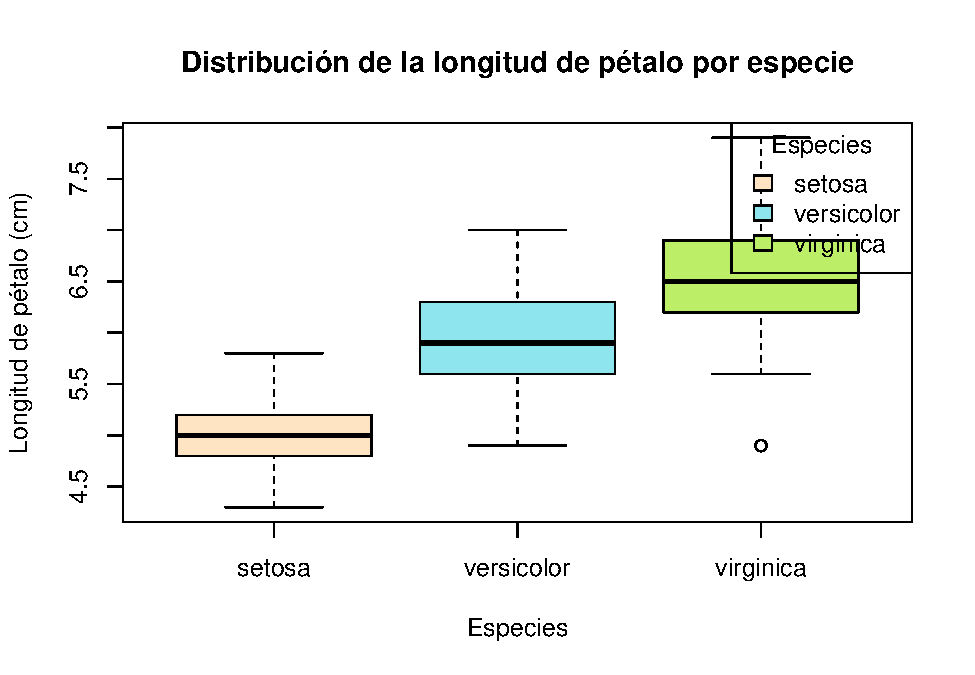
\includegraphics[keepaspectratio]{Tarea-2_files/figure-latex/unnamed-chunk-1-1.pdf}}

\begin{Shaded}
\begin{Highlighting}[]
\CommentTok{\# Versicolor y virginica {-}{-}{-}{-}{-}{-}{-}{-}{-}{-}{-}{-}{-}{-}{-}{-}{-}{-}{-}{-}{-}{-}{-}{-}{-}{-}{-}{-}{-}{-}{-}{-}{-}{-}{-}{-}{-}{-}{-}{-}{-}{-}{-}{-}{-}{-}{-}{-}{-}{-}}

\CommentTok{\# Selección de ambas especies de la base de datos}

\NormalTok{dat\_iris }\OtherTok{\textless{}{-}} \FunctionTok{subset}\NormalTok{(iris, Species }\SpecialCharTok{\%in\%} \FunctionTok{c}\NormalTok{(}\StringTok{"versicolor"}\NormalTok{,}
                                        \StringTok{"virginica"}\NormalTok{))}

\FunctionTok{View}\NormalTok{(dat\_iris) }
\NormalTok{dat\_iris}\SpecialCharTok{$}\NormalTok{Species }\OtherTok{\textless{}{-}} \FunctionTok{droplevels}\NormalTok{(dat\_iris}\SpecialCharTok{$}\NormalTok{Species) }\CommentTok{\# Para quitar "setosa" de la gráfica de la base de datos original.}
\FunctionTok{boxplot}\NormalTok{(dat\_iris}\SpecialCharTok{$}\NormalTok{Sepal.Length }\SpecialCharTok{\textasciitilde{}}\NormalTok{ dat\_iris}\SpecialCharTok{$}\NormalTok{Species,}
        \AttributeTok{xlab =} \StringTok{"Especies"}\NormalTok{,}
        \AttributeTok{ylab =} \StringTok{"Longitud de pétalo (cm)"}\NormalTok{,}
        \AttributeTok{main =} \StringTok{"Distribución de la longitud de pétalo de dos especies"}\NormalTok{,}
        \AttributeTok{col =} \FunctionTok{c}\NormalTok{(}\StringTok{"cadetblue2"}\NormalTok{, }\StringTok{"darkolivegreen2"}\NormalTok{))}
\FunctionTok{legend}\NormalTok{(}\StringTok{"topright"}\NormalTok{,}
       \AttributeTok{legend =} \FunctionTok{levels}\NormalTok{(dat\_iris}\SpecialCharTok{$}\NormalTok{Species),}
       \AttributeTok{fill =} \FunctionTok{c}\NormalTok{(}\StringTok{"cadetblue2"}\NormalTok{, }\StringTok{"darkolivegreen2"}\NormalTok{),}
       \AttributeTok{title =} \StringTok{"Especies"}\NormalTok{)}
\end{Highlighting}
\end{Shaded}

\pandocbounded{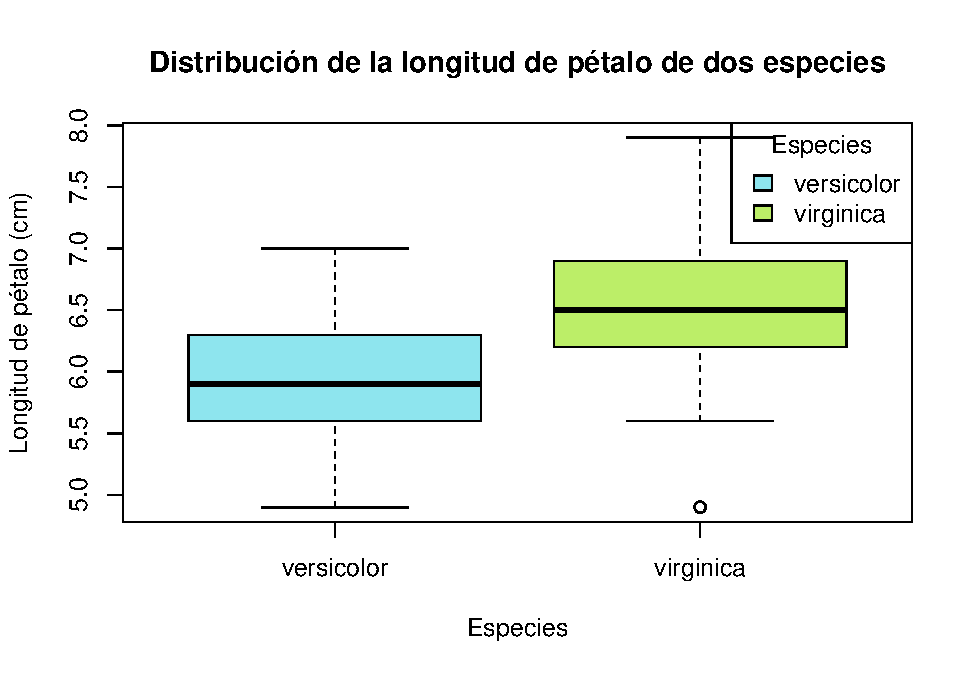
\includegraphics[keepaspectratio]{Tarea-2_files/figure-latex/unnamed-chunk-1-2.pdf}}

\begin{Shaded}
\begin{Highlighting}[]
\CommentTok{\# Prueba de T {-}{-}{-}{-}{-}{-}{-}{-}{-}{-}{-}{-}{-}{-}{-}{-}{-}{-}{-}{-}{-}{-}{-}{-}{-}{-}{-}{-}{-}{-}{-}{-}{-}{-}{-}{-}{-}{-}{-}{-}{-}{-}{-}{-}{-}{-}{-}{-}{-}{-}{-}{-}{-}{-}{-}{-}{-}{-}{-}{-}{-}}

\FunctionTok{head}\NormalTok{(dat\_iris)}
\end{Highlighting}
\end{Shaded}

\begin{verbatim}
##    Sepal.Length Sepal.Width Petal.Length Petal.Width    Species
## 51          7.0         3.2          4.7         1.4 versicolor
## 52          6.4         3.2          4.5         1.5 versicolor
## 53          6.9         3.1          4.9         1.5 versicolor
## 54          5.5         2.3          4.0         1.3 versicolor
## 55          6.5         2.8          4.6         1.5 versicolor
## 56          5.7         2.8          4.5         1.3 versicolor
\end{verbatim}

\begin{Shaded}
\begin{Highlighting}[]
\FunctionTok{summary}\NormalTok{(dat\_iris) }
\end{Highlighting}
\end{Shaded}

\begin{verbatim}
##   Sepal.Length    Sepal.Width     Petal.Length    Petal.Width   
##  Min.   :4.900   Min.   :2.000   Min.   :3.000   Min.   :1.000  
##  1st Qu.:5.800   1st Qu.:2.700   1st Qu.:4.375   1st Qu.:1.300  
##  Median :6.300   Median :2.900   Median :4.900   Median :1.600  
##  Mean   :6.262   Mean   :2.872   Mean   :4.906   Mean   :1.676  
##  3rd Qu.:6.700   3rd Qu.:3.025   3rd Qu.:5.525   3rd Qu.:2.000  
##  Max.   :7.900   Max.   :3.800   Max.   :6.900   Max.   :2.500  
##        Species  
##  versicolor:50  
##  virginica :50  
##                 
##                 
##                 
## 
\end{verbatim}

\begin{Shaded}
\begin{Highlighting}[]
\CommentTok{\# Pregunta de investigación: ¿Varía la longitud de pétalo entre la especie versicolor y virginica?}

\CommentTok{\# H0 = No existe diferencia significativa en la longitud de pétalos entre versicolor y virginica.}
\CommentTok{\# H1 = Sí existe una diferencia significativa en la longitud de pétalos entre versicolor y virginica.}

\NormalTok{versicolor }\OtherTok{\textless{}{-}} \FunctionTok{subset}\NormalTok{(dat\_iris, Species }\SpecialCharTok{==} \StringTok{"versicolor"}\NormalTok{)}\SpecialCharTok{$}\NormalTok{Petal.Length}
\NormalTok{virginica  }\OtherTok{\textless{}{-}} \FunctionTok{subset}\NormalTok{(dat\_iris, Species }\SpecialCharTok{==} \StringTok{"virginica"}\NormalTok{)}\SpecialCharTok{$}\NormalTok{Petal.Length}


\CommentTok{\# QQ{-}plot {-}{-}{-}{-}{-}{-}{-}{-}{-}{-}{-}{-}{-}{-}{-}{-}{-}{-}{-}{-}{-}{-}{-}{-}{-}{-}{-}{-}{-}{-}{-}{-}{-}{-}{-}{-}{-}{-}{-}{-}{-}{-}{-}{-}{-}{-}{-}{-}{-}{-}{-}{-}{-}{-}{-}{-}{-}{-}{-}{-}{-}{-}{-}{-}{-}}


\FunctionTok{par}\NormalTok{(}\AttributeTok{mfrow=}\FunctionTok{c}\NormalTok{(}\DecValTok{1}\NormalTok{,}\DecValTok{2}\NormalTok{))}
\FunctionTok{qqnorm}\NormalTok{(versicolor); }\FunctionTok{qqline}\NormalTok{(versicolor)}
\FunctionTok{qqnorm}\NormalTok{(virginica); }\FunctionTok{qqline}\NormalTok{(virginica)}
\end{Highlighting}
\end{Shaded}

\pandocbounded{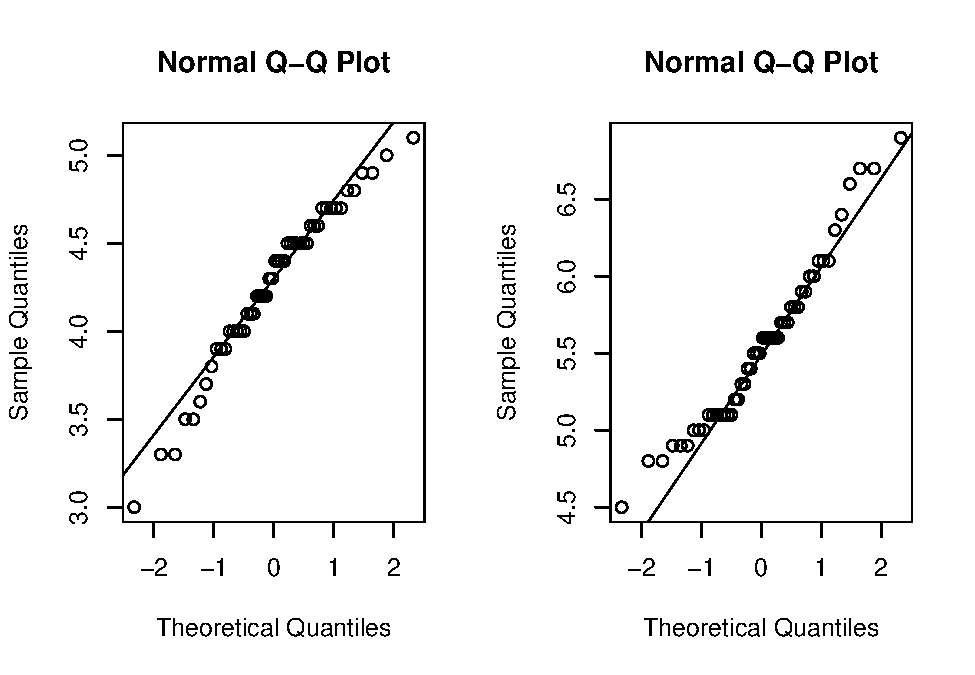
\includegraphics[keepaspectratio]{Tarea-2_files/figure-latex/unnamed-chunk-1-3.pdf}}

\begin{Shaded}
\begin{Highlighting}[]
\FunctionTok{par}\NormalTok{(}\AttributeTok{mfrow=}\FunctionTok{c}\NormalTok{(}\DecValTok{1}\NormalTok{,}\DecValTok{2}\NormalTok{))}

\CommentTok{\# Normalidad {-}{-}{-}{-}{-}{-}{-}{-}{-}{-}{-}{-}{-}{-}{-}{-}{-}{-}{-}{-}{-}{-}{-}{-}{-}{-}{-}{-}{-}{-}{-}{-}{-}{-}{-}{-}{-}{-}{-}{-}{-}{-}{-}{-}{-}{-}{-}{-}{-}{-}{-}{-}{-}{-}{-}{-}{-}{-}{-}{-}{-}{-}}

\CommentTok{\# Normalidad ✅}

\FunctionTok{shapiro.test}\NormalTok{(versicolor) }\CommentTok{\# p{-}value = 0.1585}
\end{Highlighting}
\end{Shaded}

\begin{verbatim}
## 
##  Shapiro-Wilk normality test
## 
## data:  versicolor
## W = 0.966, p-value = 0.1585
\end{verbatim}

\begin{Shaded}
\begin{Highlighting}[]
\FunctionTok{shapiro.test}\NormalTok{(virginica) }\CommentTok{\#  p{-}value = 0.1098}
\end{Highlighting}
\end{Shaded}

\begin{verbatim}
## 
##  Shapiro-Wilk normality test
## 
## data:  virginica
## W = 0.96219, p-value = 0.1098
\end{verbatim}

\begin{Shaded}
\begin{Highlighting}[]
\CommentTok{\# Varianza {-}{-}{-}{-}{-}{-}{-}{-}{-}{-}{-}{-}{-}{-}{-}{-}{-}{-}{-}{-}{-}{-}{-}{-}{-}{-}{-}{-}{-}{-}{-}{-}{-}{-}{-}{-}{-}{-}{-}{-}{-}{-}{-}{-}{-}{-}{-}{-}{-}{-}{-}{-}{-}{-}{-}{-}{-}{-}{-}{-}{-}{-}{-}{-}}

\CommentTok{\# Varianza ✅}

\FunctionTok{var.test}\NormalTok{(versicolor, virginica) }\CommentTok{\# df = 49, p{-}value = 0.2637}
\end{Highlighting}
\end{Shaded}

\begin{verbatim}
## 
##  F test to compare two variances
## 
## data:  versicolor and virginica
## F = 0.72497, num df = 49, denom df = 49, p-value = 0.2637
## alternative hypothesis: true ratio of variances is not equal to 1
## 95 percent confidence interval:
##  0.411402 1.277530
## sample estimates:
## ratio of variances 
##          0.7249678
\end{verbatim}

\begin{Shaded}
\begin{Highlighting}[]
\CommentTok{\# Homogeneidad {-}{-}{-}{-}{-}{-}{-}{-}{-}{-}{-}{-}{-}{-}{-}{-}{-}{-}{-}{-}{-}{-}{-}{-}{-}{-}{-}{-}{-}{-}{-}{-}{-}{-}{-}{-}{-}{-}{-}{-}{-}{-}{-}{-}{-}{-}{-}{-}{-}{-}{-}{-}{-}{-}{-}{-}{-}{-}{-}{-}}

\CommentTok{\# Homogeneidad ✅}

\FunctionTok{var.test}\NormalTok{(versicolor, virginica, }\AttributeTok{alternative =} \StringTok{"two.sided"}\NormalTok{)}
\end{Highlighting}
\end{Shaded}

\begin{verbatim}
## 
##  F test to compare two variances
## 
## data:  versicolor and virginica
## F = 0.72497, num df = 49, denom df = 49, p-value = 0.2637
## alternative hypothesis: true ratio of variances is not equal to 1
## 95 percent confidence interval:
##  0.411402 1.277530
## sample estimates:
## ratio of variances 
##          0.7249678
\end{verbatim}

\begin{Shaded}
\begin{Highlighting}[]
\CommentTok{\# Prueba t de Student {-}{-}{-}{-}{-}{-}{-}{-}{-}{-}{-}{-}{-}{-}{-}{-}{-}{-}{-}{-}{-}{-}{-}{-}{-}{-}{-}{-}{-}{-}{-}{-}{-}{-}{-}{-}{-}{-}{-}{-}{-}{-}{-}{-}{-}{-}{-}{-}{-}{-}{-}{-}{-}}

\CommentTok{\# Prueba t de Student}

\FunctionTok{t.test}\NormalTok{(versicolor, virginica,}
       \AttributeTok{alternative =} \StringTok{"two.sided"}\NormalTok{,}
       \AttributeTok{var.equal =}\NormalTok{ T)}
\end{Highlighting}
\end{Shaded}

\begin{verbatim}
## 
##  Two Sample t-test
## 
## data:  versicolor and virginica
## t = -12.604, df = 98, p-value < 2.2e-16
## alternative hypothesis: true difference in means is not equal to 0
## 95 percent confidence interval:
##  -1.495426 -1.088574
## sample estimates:
## mean of x mean of y 
##     4.260     5.552
\end{verbatim}

\begin{Shaded}
\begin{Highlighting}[]
\CommentTok{\# p{-}value \textless{} 2.2e{-}16 = 0.00000000000000022 }

\CommentTok{\# **Se rechaza la H0 y se acepta la H1.**}


\CommentTok{\# Cohen´s effect {-}{-}{-}{-}{-}{-}{-}{-}{-}{-}{-}{-}{-}{-}{-}{-}{-}{-}{-}{-}{-}{-}{-}{-}{-}{-}{-}{-}{-}{-}{-}{-}{-}{-}{-}{-}{-}{-}{-}{-}{-}{-}{-}{-}{-}{-}{-}{-}{-}{-}{-}{-}{-}{-}{-}{-}{-}{-}}

\CommentTok{\# Cohen´s effect ✅⬆️}

\NormalTok{cohens\_efecto }\OtherTok{\textless{}{-}} \ControlFlowTok{function}\NormalTok{(x, y) \{}
\NormalTok{  n1 }\OtherTok{\textless{}{-}} \FunctionTok{length}\NormalTok{(x); n2 }\OtherTok{\textless{}{-}} \FunctionTok{length}\NormalTok{(y)}
\NormalTok{  s1 }\OtherTok{\textless{}{-}} \FunctionTok{sd}\NormalTok{(x); s2 }\OtherTok{\textless{}{-}} \FunctionTok{sd}\NormalTok{(y)}
\NormalTok{  sp }\OtherTok{\textless{}{-}} \FunctionTok{sqrt}\NormalTok{(((n1 }\SpecialCharTok{{-}} \DecValTok{1}\NormalTok{) }\SpecialCharTok{*}\NormalTok{ s1}\SpecialCharTok{\^{}}\DecValTok{2} \SpecialCharTok{+}\NormalTok{ (n2 }\SpecialCharTok{{-}} \DecValTok{1}\NormalTok{) }\SpecialCharTok{*}\NormalTok{ s2}\SpecialCharTok{\^{}}\DecValTok{2}\NormalTok{) }\SpecialCharTok{/}\NormalTok{ (n1 }\SpecialCharTok{+}\NormalTok{ n2 }\SpecialCharTok{{-}} \DecValTok{2}\NormalTok{))}
\NormalTok{  (}\FunctionTok{mean}\NormalTok{(x) }\SpecialCharTok{{-}} \FunctionTok{mean}\NormalTok{(y)) }\SpecialCharTok{/}\NormalTok{ sp}
\NormalTok{\}}


\NormalTok{d1\_cal }\OtherTok{\textless{}{-}} \FunctionTok{cohens\_efecto}\NormalTok{(versicolor,virginica)}
\NormalTok{d1\_cal}
\end{Highlighting}
\end{Shaded}

\begin{verbatim}
## [1] -2.520756
\end{verbatim}

\begin{Shaded}
\begin{Highlighting}[]
\CommentTok{\# Cohen´s effect = {-}2.520756 lo que nos dice que es un efecto muy grande. }


\CommentTok{\# Visualización {-}{-}{-}{-}{-}{-}{-}{-}{-}{-}{-}{-}{-}{-}{-}{-}{-}{-}{-}{-}{-}{-}{-}{-}{-}{-}{-}{-}{-}{-}{-}{-}{-}{-}{-}{-}{-}{-}{-}{-}{-}{-}{-}{-}{-}{-}{-}{-}{-}{-}{-}{-}{-}{-}{-}{-}{-}{-}{-}}

\FunctionTok{library}\NormalTok{(ggplot2)}
\NormalTok{dat\_sub }\OtherTok{\textless{}{-}} \FunctionTok{subset}\NormalTok{(dat\_iris, Species }\SpecialCharTok{\%in\%} \FunctionTok{c}\NormalTok{(}\StringTok{"versicolor"}\NormalTok{, }\StringTok{"virginica"}\NormalTok{))}

\FunctionTok{ggplot}\NormalTok{(dat\_sub, }\FunctionTok{aes}\NormalTok{(}\AttributeTok{x =}\NormalTok{ Species, }\AttributeTok{y =}\NormalTok{ Petal.Length, }\AttributeTok{fill =}\NormalTok{ Species)) }\SpecialCharTok{+}
  \FunctionTok{geom\_violin}\NormalTok{(}\AttributeTok{trim =} \ConstantTok{FALSE}\NormalTok{, }\AttributeTok{color =} \StringTok{"black"}\NormalTok{, }\AttributeTok{alpha =} \FloatTok{0.6}\NormalTok{) }\SpecialCharTok{+} 
  \FunctionTok{geom\_boxplot}\NormalTok{(}\AttributeTok{width =} \FloatTok{0.1}\NormalTok{, }\AttributeTok{fill =} \StringTok{"white"}\NormalTok{, }\AttributeTok{outlier.shape =} \ConstantTok{NA}\NormalTok{) }\SpecialCharTok{+}
  \FunctionTok{stat\_summary}\NormalTok{(}\AttributeTok{fun =}\NormalTok{ mean, }\AttributeTok{geom =} \StringTok{"point"}\NormalTok{, }\AttributeTok{shape =} \DecValTok{23}\NormalTok{, }\AttributeTok{size =} \DecValTok{3}\NormalTok{, }\AttributeTok{fill =} \StringTok{"red"}\NormalTok{) }\SpecialCharTok{+}
  \FunctionTok{theme\_minimal}\NormalTok{() }\SpecialCharTok{+}
  \FunctionTok{labs}\NormalTok{(}\AttributeTok{title =} \StringTok{"Distribución de la longitud de pétalos por especie"}\NormalTok{,}
       \AttributeTok{x =} \StringTok{"Especie"}\NormalTok{,}
       \AttributeTok{y =} \StringTok{"Longitud de pétalo (cm)"}\NormalTok{) }\SpecialCharTok{+}
  \FunctionTok{theme}\NormalTok{(}\AttributeTok{legend.position =} \StringTok{"none"}\NormalTok{)}
\end{Highlighting}
\end{Shaded}

\pandocbounded{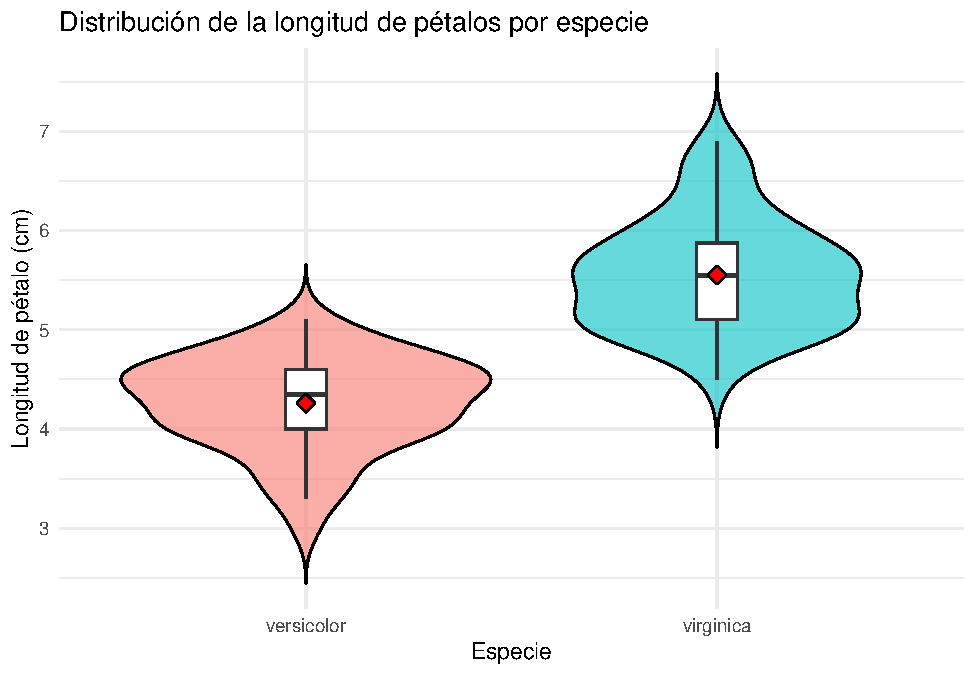
\includegraphics[keepaspectratio]{Tarea-2_files/figure-latex/unnamed-chunk-1-4.pdf}}

\end{document}
